% !TEX root = ./main.tex
% Loop Optimizations
% ======================================================
\par \noindent 支配节点(Dominators):若 $d$ 支配 $n$,则从流图的入口 $s_0$ 到节点 $n$ 的每条路径都经过节点 $d$。
计算支配 $n$ 的所有节点 $D[n]$:$D(n) = \{n\} \cup \bigcap_{p \in \text{pred}(n)} D[p]$,初始条件:$D[s_0] = \{s_0\}$。
\par \noindent 直接支配结点(immediate dominator):支配节点集合中除了 $n$ 本身的最接近 $n$ 的节点。
\par \noindent 支配节点树(dominator tree):树中一个节点的子节点是该节点的直接支配节点。每个结点只支配它和它的后代结点。

\par \noindent Back Edge:当 $h$ 支配 $n$ 时从 $n$ 到 $h$ 的边。
Back Edge $n \rightarrow h$ 的自然循环是满足以下条件的节点 $x$ 的集合:1.$h$ 支配 $x$;2. 有一条从 $x$ 到 $n$ 的路径不包含 $h$。
自然循环满足性质:1. 有唯一的入口结点,称为首结点(header);2. 首结点支配循环中的所有结点;3. 循环中至少有一条返回首结点的路径;
4. 除非两个自然循环的首结点相同,否则,它们要么互不相交,要么一个完全包含在另外一个里面。
\par \noindent 循环嵌套树(Loop-Nest Tree):树的叶节点是最内层循环。构造:
1. 画出支配节点树;
2. 找到所有自然循环,并找到所有循环首结点;
3. 对于每个循环首结点 $h$,将 $h$ 的所有自然循环合并为一个循环 $\text{loop}[h]$,循环中的节点写在第二行,首节点写在第一行;
4. 如果 $h_2$ 在循环 $\text{loop}[h_1]$ 中,那么 $h1$ 在循环嵌套树中高于 $h_2$。

\begin{figure}[H]
    \centering
    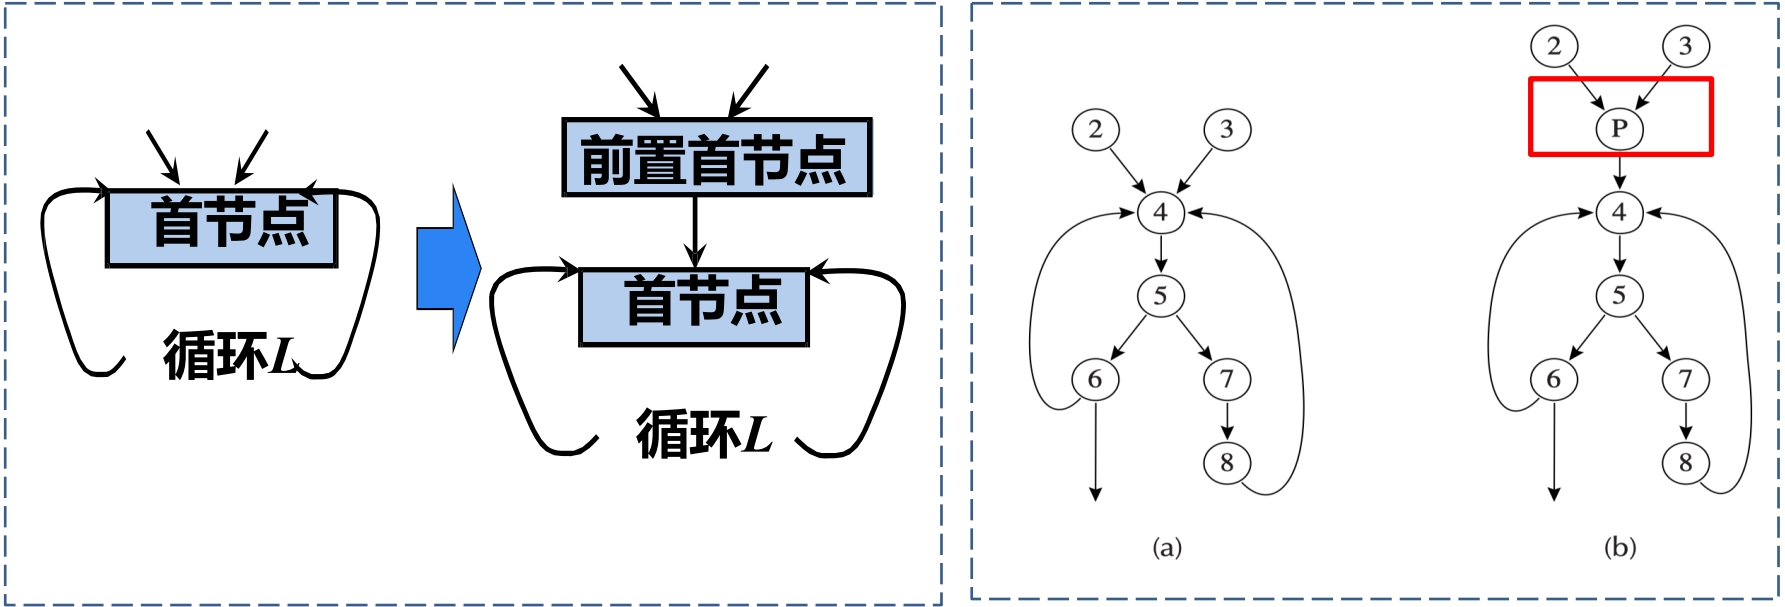
\includegraphics[width=0.8\linewidth]{figures/loop1.png}
\end{figure}

\par \noindent 循环不变式(Loop Invariant):在循环中,每次迭代都保持不变的量。循环不变式的生成:
表达式 \texttt{x := v1 op v2} 是循环 $L$ 中的不变式,当且仅当:(基础情况)it’s a constant 或者 
it’s a variable use, all of whose defs are outside of $L$;
(归纳情况)it’s a pure computation all of whose arguments are loop-invariant 或者
it’s a variable use with only one reaching def, and the rhs of that def is loop-invariant。

\par \noindent 提升(Hoist) \texttt{d : t <- a op b} 到循环的前置首节点(preheader)末尾的条件:
1. $d$ dominates all loop exits where $t$ is live-out(很可能阻止许多计算从 while 循环中提升);
2. and there is only one definition of $t$ in the loop;
3. and $t$ is not live-out of the loop preheader (that is, $t$ is not live before the loop)。
如果 \texttt{d : t <- a op b} 可能引起某种算术异常或产生其他副作用,则需要修改这些规则。